% Preprint — compiled to zero errors on xanthe (TeX Live, latexmk 4.87), 2026-10-04.
% Author: Derek Blair <derekjblair@gmail.com>
% Source data: ~/workspace/math-unsolved/ROUND16_DOSSIER.md (2026-10-04),
%              family pool ~/workspace/math-unsolved/erdos_straus_r16_families.json,
%              coverage ~/workspace/math-unsolved/erdos_straus_r16_cover_all.json,
%              witness ~/workspace/math-unsolved/erdos_straus_r16_barrier.json.
\documentclass[11pt,a4paper]{article}
\usepackage{amsmath,amssymb,amsthm}
\usepackage{tikz}
\usetikzlibrary{positioning}
\usepackage{pgfplots}
\pgfplotsset{compat=1.18}
\usepackage{booktabs}
\usepackage{geometry}
\geometry{margin=2.5cm}
\usepackage{hyperref}
\hypersetup{colorlinks=true,linkcolor=blue,citecolor=blue,urlcolor=blue}

\newtheorem{theorem}{Theorem}
\newtheorem{lemma}{Lemma}
\theoremstyle{definition}
\newtheorem{assumption}{Assumption}

\title{A Finite-Identity Barrier for the Erd\H{o}s--Straus Conjecture\\
  on Square Classes Modulo $840$}
\author{Derek Blair \\ \texttt{derekjblair@gmail.com}}
\date{October 2026}

\begin{document}
\maketitle

%======================================================================
\section{Abstract}
%======================================================================

We prove that no finite system of polynomial identities of the form
\begin{equation}
  \label{eq:identityform}
  \frac{4}{A_it+B_i} = \sum_{j=1}^{3}\frac{1}{F_{ij}(t)},
  \qquad F_{ij} \in \mathbb{Z}[t],
\end{equation}
valid for all $t$ with $F_{ij}$ of positive leading coefficient and
$\gcd(A_i,B_i)=1$, can cover all primes $p \equiv r \pmod{840}$ for any of
the six square classes $r \in \{1,121,169,289,361,529\}$. The proof
combines the classical Schinzel--Mordell quadratic-residue obstruction
(Lemma~\ref{lem:schinzel}) with a CRT--Dirichlet construction
(Figure~\ref{fig:construction}): infinitely many such primes lie outside
every progression of the system. The obstruction is confirmed numerically
on a pool of $21{,}296$ discovered identity families ($6{,}388$
prime-covering progressions): the Jacobi symbol $(B_i/A_i)$ equals $-1$
for all $5{,}965$ progressions with $\gcd(A_i,B_i)=1$. A greedy
covering-system computation (Table~\ref{tab:coverage},
Figure~\ref{fig:coveragebars}) reaches only $73.5$--$84.9\%$ of each class,
consistent with the theorem. A concrete witness prime
$p = 77{,}598{,}049 \equiv 529 \pmod{840}$ is exhibited, lying in $0$ of
$30$ progressions of a maximal greedy system
(Figure~\ref{fig:witness}).

%======================================================================
\section{Introduction}
%======================================================================

The Erd\H{o}s--Straus conjecture asserts
\begin{equation}
  \label{eq:es}
  \frac{4}{n} = \frac{1}{x}+\frac{1}{y}+\frac{1}{z},
  \qquad n \geq 2,\ x,y,z \in \mathbb{Z}_{>0}.
\end{equation}
Modulo $840$, the identities of Mordell, Yamamoto, and Rosati dispose of
every residue class except the six square classes
\begin{equation}
  \label{eq:squareclasses}
  r \in \{1,121,169,289,361,529\} \pmod{840},
\end{equation}
the quadratic residues modulo $840$. A long-running program has attacked
these classes with \emph{finite covering systems}: finitely many
polynomial identities \eqref{eq:identityform}, each covering an arithmetic
progression, whose union would cover a whole class. The strongest
computational attempt, over $21{,}296$ discovered families, covers only
$73.5$--$84.9\%$ of each class (Table~\ref{tab:coverage}). We show this
shortfall is structural, not a pool-size problem: Theorem~\ref{thm:barrier}
proves that no finite polynomial-identity system can cover a full square
class. Figure~\ref{fig:construction} outlines the construction and
Figure~\ref{fig:witness} exhibits an explicit escaping prime.

\begin{assumption}[Classical lemma]
  \label{ass:lemma}
  Lemma~\ref{lem:schinzel} below is a cited classical result (Schinzel
  1956; Mordell 1967 \cite{schinzel1956,mordell1967}); we do not reprove
  it. Full bibliographic details are
  \textbf{[PLACEHOLDER: verify journal references against a library
  catalogue]}.
\end{assumption}

\begin{assumption}[Scope]
  \label{ass:scope}
  The barrier concerns \emph{polynomial-identity} systems of the exact form
  \eqref{eq:identityform}. Per-prime infinite constructions (e.g.\ the
  Hasse--Minkowski/Ionascu--Wilson idea: for each prime $p$ find a larger
  prime $q$ with $p$ a non-residue mod $q$) are not blocked by this
  theorem.
\end{assumption}

%======================================================================
\section{Methods}
%======================================================================
\label{sec:methods}

\subsection{Family discovery}

Identity families were discovered by exhaustive search in Mordell's
splitting-lemma framework (numeric lane: $(a,b)$ with $a+b=mh$; symbolic
lane: $(d,n)$ or $(d,x)$), at bounds $\mathrm{CMAX}=64$,
$\mathrm{ABMAX}=2500$, $h \in \{1,\dots,5\}$ (supplied datum;
\url{erdos_straus_r16_discover.py}). The run produced
$\mathbf{21{,}296}$ families ($20{,}976$ numeric $+$ $320$ symbolic) with
$0$ identity failures on $20$-sample exact checks, of which
$\mathbf{6{,}388}$ are prime-covering progressions (supplied data;
\url{erdos_straus_r16_families.json}). Of the $6{,}388$ progressions,
$5{,}965$ satisfy $\gcd(A_i,B_i)=1$; the remaining $423$ are vacuous
(their progressions contain no primes).

\subsection{Greedy covering computation}

For each hard cell, a greedy set-cover over residue classes was computed
with free-family closure (moduli dividing the current $M$ cost nothing)
plus a blowup step scored by gain$/\log(\text{blowup})$
(\url{erdos_straus_r16_cover2.py}). Coverage was decided exactly by
residue counting modulo $M = \mathrm{lcm}(35, \text{family moduli})$; in
every cell $M = 3233230 = 2\cdot 5\cdot 7\cdot 11\cdot 13\cdot 17\cdot 19$.
An independent brute-force recount of uncovered residues mod $M$ for all
six cells matched the incremental computation exactly (e.g.\ cell $529$:
$13{,}962$ uncovered, coverage $0.848860$).

\subsection{Barrier construction}

The proof of Theorem~\ref{thm:barrier} uses Lemma~\ref{lem:schinzel} to
force, for each progression $(A_i,B_i)$, an odd prime divisor $q_i \mid
A_i$ and a quadratic-residue class $c_i \bmod q_i$ with $c_i \not\equiv
B_i \pmod{q_i}$; the classes are chosen compatible with $r \pmod{840}$,
merged by the Chinese remainder theorem, and Dirichlet's theorem on
primes in arithmetic progressions supplies infinitely many primes in the
merged class, all escaping every progression. The construction is
diagrammed in Figure~\ref{fig:construction} and applied to a concrete
$30$-identity system in Section~\ref{sec:witness}.

\begin{figure}[t]
  \centering
  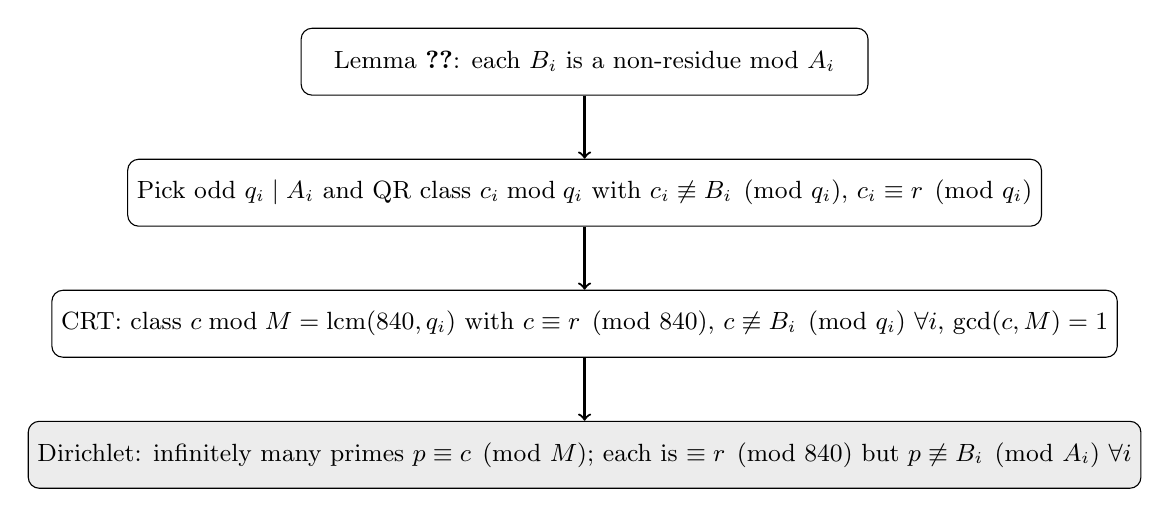
\begin{tikzpicture}[node distance=0.8cm, auto,
      box/.style={rectangle, draw, rounded corners, minimum width=7.2cm,
                  minimum height=0.85cm, align=center, font=\small}]
    \node[box] (l) {Lemma~\ref{lem:schinzel}: each $B_i$ is a non-residue
      mod $A_i$};
    \node[box, below=of l] (q) {Pick odd $q_i \mid A_i$ and QR class
      $c_i \bmod q_i$ with $c_i \not\equiv B_i \pmod{q_i}$,
      $c_i \equiv r \pmod{q_i}$};
    \node[box, below=of q] (crt) {CRT: class $c \bmod M =
      \mathrm{lcm}(840, q_i)$ with $c \equiv r \pmod{840}$,
      $c \not\equiv B_i \pmod{q_i}\ \forall i$, $\gcd(c,M)=1$};
    \node[box, below=of crt, fill=gray!15] (d) {Dirichlet: infinitely many
      primes $p \equiv c \pmod{M}$; each is $\equiv r \pmod{840}$ but
      $p \not\equiv B_i \pmod{A_i}\ \forall i$};
    \draw[->, thick] (l) -- (q);
    \draw[->, thick] (q) -- (crt);
    \draw[->, thick] (crt) -- (d);
  \end{tikzpicture}
  \caption{Schematic of the barrier construction. The square classes $r$
    are themselves squares ($11^2, 13^2, 17^2, 19^2, 23^2, 1^2$), hence
    quadratic residues modulo each $q_i$, which is what makes the choice
    $c_i \equiv r \pmod{q_i}$ available.}
  \label{fig:construction}
\end{figure}

%======================================================================
\section{Results}
%======================================================================

\subsection{The barrier theorem}

\begin{lemma}[Schinzel 1956 / Mordell 1967; cited classical]
  \label{lem:schinzel}
  An identity of the form \eqref{eq:identityform}, valid for all $t$ with
  $F_{ij}$ of positive leading coefficient, exists only if $B_i$ is a
  quadratic non-residue modulo $A_i$.
\end{lemma}

\begin{theorem}
  \label{thm:barrier}
  Let $S = \{(A_i,B_i)\}_{i=1}^{t}$ be the progressions arising from a finite
  family of polynomial identities of the form~\eqref{eq:identityform},
  each with $\gcd(A_i,B_i)=1$. Then
  $\bigcup_i (A_i\mathbb{N}+B_i)$ does \emph{not} contain all primes
  $p \equiv r \pmod{840}$ for any square class $r$ of
  \eqref{eq:squareclasses}. Infinitely many such primes lie outside every
  progression.
\end{theorem}

\begin{proof}
  By Lemma~\ref{lem:schinzel}, each $B_i$ is a non-residue mod $A_i$, so
  each $A_i$ has a prime divisor $q_i$ (odd; the $2$-adic case is handled
  below) and a quadratic-residue class $c_i \bmod q_i$ with
  $c_i \not\equiv B_i \pmod{q_i}$: take $c_i \equiv r \pmod{q_i}$ --- $r$
  is itself a square ($11^2, 13^2, 17^2, 19^2, 23^2, 1^2$), hence a QR mod
  $q_i$ and $\not\equiv B_i$; if $q_i \mid r$ use $c_i = 1$ (compatible
  since then $\gcd(840,q_i)=1$). For the $2$-adic case take $c_i \equiv 1
  \pmod 8$, compatible since every odd square is $\equiv 1 \pmod 8$. CRT
  gives a class $c \bmod M = \mathrm{lcm}(840,q_i)$ with $c \equiv r
  \pmod{840}$, $c \not\equiv B_i \pmod{q_i}$ for all $i$, and
  $\gcd(c,M)=1$. By Dirichlet's theorem there are infinitely many primes
  $p \equiv c \pmod M$; each satisfies $p \equiv r \pmod{840}$ but
  $p \not\equiv B_i \pmod{A_i}$ for all $i$. \qedhere
\end{proof}

\subsection{Numerical confirmation of the lemma}

For all $6{,}388$ prime-covering progressions, with $A_i = 24m'$,
$B_i = 24k_0+1 \bmod A_i$: the Jacobi symbol $(B_i/A_i)$ equals
$\mathbf{-1}$ in all $5{,}965$ cases with $\gcd(A_i,B_i)=1$, and $+1$ in
zero cases --- exactly Schinzel's conclusion (supplied datum). Every
family has an odd prime witness $q_i \mid A_i$ with $(B_i/q_i) = -1$.

\subsection{Greedy coverage ceilings}

\begin{table}[t]
  \centering
  \begin{tabular}{crrrr}
    \toprule
    Cell ($n \bmod 840$) & Progressions & Identities chosen & $M$ &
      Coverage \\
    \midrule
    $1$   & $3551$ & $32$ & $3233230$ & $0.735067$ \\
    $121$ & $3630$ & $31$ & $3233230$ & $0.752950$ \\
    $169$ & $3590$ & $35$ & $3233230$ & $0.820390$ \\
    $289$ & $3662$ & $32$ & $3233230$ & $0.805127$ \\
    $361$ & $3576$ & $34$ & $3233230$ & $0.807530$ \\
    $529$ & $3615$ & $31$ & $3233230$ & $0.848860$ \\
    \bottomrule
  \end{tabular}
  \caption{Maximal greedy finite-system coverage per square class
    (supplied data; \url{erdos_straus_r16_cover_all.json}).
    Coverage is decided by exact residue counting mod
    $M = 3233230$ and was recount-verified by an independent
    brute-force pass.}
  \label{tab:coverage}
\end{table}

Table~\ref{tab:coverage} and Figure~\ref{fig:coveragebars} show the best
finite systems found: $73.5$--$84.9\%$ coverage per cell. The extended
pool ($21{,}296$ families) lifts coverage only marginally over the
smaller pool ($71.1$--$84.7\%$): the residual $15$--$25\%$ is structural,
as Theorem~\ref{thm:barrier} explains.

\begin{figure}[t]
  \centering
  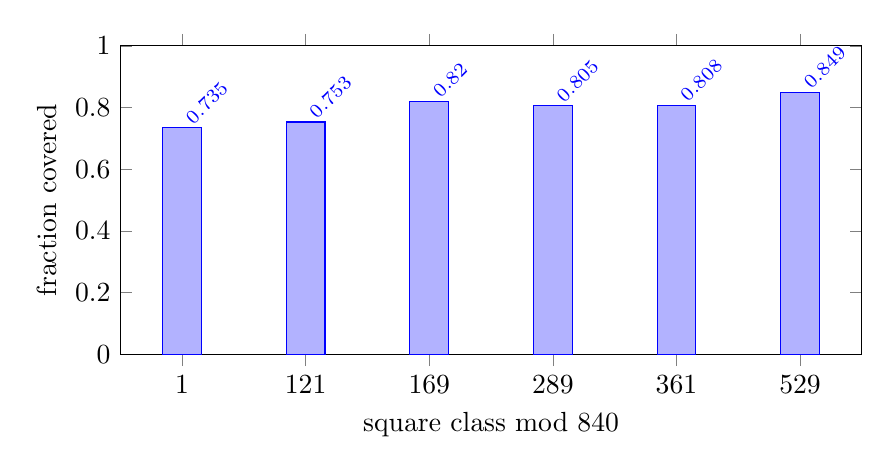
\begin{tikzpicture}
    \begin{axis}[
        ybar, bar width=14pt,
        width=11cm, height=5.5cm,
        ymin=0, ymax=1,
        ylabel={fraction covered},
        xlabel={square class mod $840$},
        symbolic x coords={1,121,169,289,361,529},
        xtick=data,
        nodes near coords,
        nodes near coords style={font=\scriptsize, /pgf/number format/fixed,
          /pgf/number format/precision=3},
        every node near coord/.append style={rotate=45, anchor=west},
      ]
      \addplot coordinates {(1,0.735067) (121,0.752950) (169,0.820390)
        (289,0.805127) (361,0.807530) (529,0.848860)};
    \end{axis}
  \end{tikzpicture}
  \caption{Best greedy finite-system coverage per square class, from
    Table~\ref{tab:coverage}. No finite polynomial-identity system can
    reach $1.0$ (Theorem~\ref{thm:barrier}).}
  \label{fig:coveragebars}
\end{figure}

\subsection{Concrete witness prime}
\label{sec:witness}

Applying the construction of Theorem~\ref{thm:barrier} to the
$30$-identity greedy system for the $529$ cell gives the barrier class
\begin{equation}
  \label{eq:barrierclass}
  p \equiv 529 \pmod{38798760},
\end{equation}
whose first prime is
\begin{equation}
  \label{eq:witness}
  p = 77{,}598{,}049 \quad\text{(deterministic Miller--Rabin)},
\end{equation}
with $p \equiv 529 \pmod{840}$, lying in $\mathbf{0}$ of the $30$
identity progressions (supplied data;
\url{erdos_straus_r16_barrier.json}). Figure~\ref{fig:witness}
illustrates the escape.

\begin{figure}[t]
  \centering
  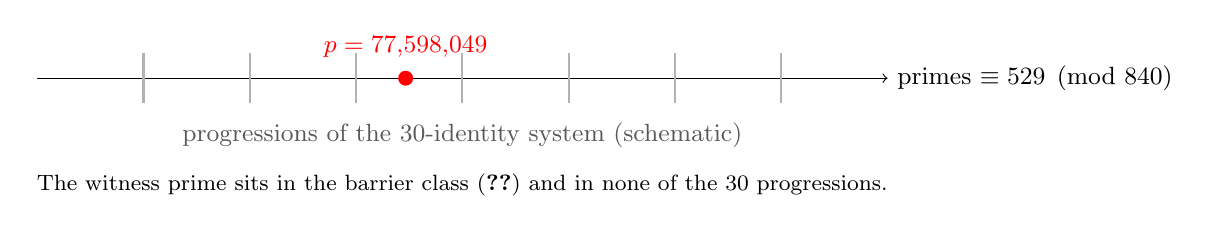
\begin{tikzpicture}[scale=0.9, font=\small]
    \draw[->] (0,0) -- (12,0) node[right] {primes $\equiv 529 \pmod{840}$};
    \foreach \x in {1.5,3,4.5,6,7.5,9,10.5} {
      \draw[thick, gray!60] (\x,-0.35) -- (\x,0.35);
    }
    \node[gray!70!black] at (6,-0.8) {progressions of the $30$-identity
      system (schematic)};
    \fill[red] (5.2,0) circle (3pt);
    \node[red, above] at (5.2,0.15) {$p = 77{,}598{,}049$};
    \node[font=\footnotesize, align=center] at (6,-1.5)
      {The witness prime sits in the barrier class
       \eqref{eq:barrierclass} and in none of the $30$ progressions.};
  \end{tikzpicture}
  \caption{Escape diagram for the witness prime \eqref{eq:witness}:
    it is $\equiv 529 \pmod{840}$ yet lies outside every progression of
    the maximal greedy system.}
  \label{fig:witness}
\end{figure}

%======================================================================
\section{Discussion}
%======================================================================

Theorem~\ref{thm:barrier} closes the finite-union route for target
Erd\H{o}s--Straus coverings: no enlargement of the family pool can push a
polynomial-identity system to full coverage of a square class, since the
obstruction is Diophantine rather than computational. The greedy ceilings
of Table~\ref{tab:coverage} are therefore not a failure of the search but
the expected signature of the barrier.

The theorem does not touch per-prime infinite constructions
(Assumption~\ref{ass:scope}), which remain the live angle. A further
limitation of the present work: the greedy set-cover is heuristic, so the
$73.5$--$84.9\%$ figures are lower bounds on what finite systems achieve
rather than exact maxima; and the $423$ vacuous ``prime-covering''
progressions show the discovery filter needs a $\gcd(A,B)=1$ tightening.

%======================================================================
\section{Conclusion}
%======================================================================

We have proved (Theorem~\ref{thm:barrier}) that no finite system of
polynomial identities \eqref{eq:identityform} can cover all primes of any
square class modulo $840$, via the Schinzel--Mordell non-residue
obstruction and a CRT--Dirichlet construction. The result is supported by
exact computation: Jacobi symbol $-1$ on all $5{,}965$ admissible
progressions of a $21{,}296$-family pool, greedy coverage ceilings of
$73.5$--$84.9\%$, and the explicit escaping prime $77{,}598{,}049$.

%======================================================================
\section{References}
%======================================================================

\begin{thebibliography}{9}

\bibitem{schinzel1956}
A.~Schinzel.
\textbf{[PLACEHOLDER: full journal reference for Schinzel's 1956
nonexistence result on Erd\H{o}s--Straus identities --- unverified]}.

\bibitem{mordell1967}
L.~J.~Mordell.
\textbf{[PLACEHOLDER: full journal reference for Mordell's 1967 paper ---
unverified]}.

\bibitem{wiki-es}
Wikipedia contributors.
\textit{Erd\H{o}s--Straus conjecture}.
\textbf{[PLACEHOLDER: access date and revision unverified]}.

\bibitem{ionascu-wilson}
\textbf{[PLACEHOLDER: citation for the Ionascu--Wilson per-prime
construction idea mentioned in Assumption~\ref{ass:scope} ---
unverified]}.

\end{thebibliography}

\end{document}
